\documentclass[svgnames]{beamer}

\usepackage{pri}
\usepackage{comment}
\usepackage{pstricks}
\usepackage{pst-node}
\usepackage{pst-plot}

\SpecialCoor 

\newcommand{\wij}{\ensuremath{w_{i,j}}}

% as figuras podem estar numa destas pastas:
\graphicspath{{./}{figures/}{figures/03-IR-models-figs/}{figures/02-intro-IR/}}

\title{Processamento e Recuperação de Informação}

\subtitle{Information Retrieval Models}

%%% algumas frames formatam pslatex; 
%%% no aquamacs trocar com " ^C ^T ^P	TeX-PDF-mode"

\begin{document}

\maketitle
\makeoutline

\begin{frame} \frametitle{Bibliography}

    \begin{block}{}
      \href{http://www.mir2ed.org/}{Ricardo Baeza-Yates,
            Berthier Ribeiro-Neto, Modern Information Retrieval, 2nd
            edtion}. Chapter 3
    \end{block}

    \begin{block}{}
      \href{http://nlp.stanford.edu/IR-book/}{Christopher D. Manning, Prabhakar Raghavan and Hinrich Schütze, Introduction to Information Retrieval}. Chapters 1, 6, 11 and 12
    \end{block}
    
        \begin{block}{}
      \href{https://www.cs.uic.edu/~liub/WebMiningBook.html}{Bing Liu, Web Data Mining - Exploring Hyperlinks, Contents, and Usage Data.} Chapter 6.
    \end{block}
    

\end{frame}

\section{Generic Document Model}

\begin{frame}
  \frametitle{Retrieval Models}

  \begin{center}
    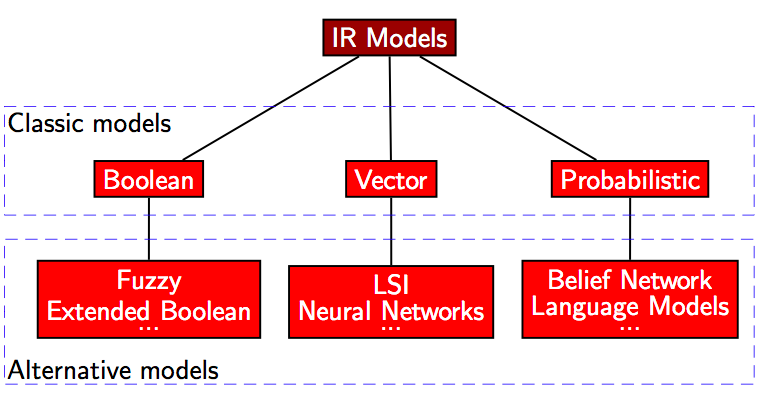
\includegraphics[width=.8\linewidth]{retrieval-models.png}\\
  \end{center}

\end{frame}

\begin{frame} \frametitle{Index Terms}
  
  \begin{block}{}
    In the classic IR models, documents are represented by \\
    \emph{index terms}
      \begin{itemize}
      \item full text/selected keywords
      \item structure/no structure
      \end{itemize}
   \end{block}

  \begin{block}{}
      Not all terms are equally useful
      \begin{itemize}
      \item index terms can be \emph{weighted}
      \end{itemize}
   \end{block}

  \begin{block}{}
    We assume that terms are \emph{mutually independent}
      \begin{itemize}
      \item this is, of course, a simplification
      \end{itemize}
  \end{block}

\end{frame}

\begin{frame} \frametitle{Definition of a Document Model}
  
  \begin{definition}
    Let $t$ be the number of index terms in the collection of documents, and
    let $k_i$ be a generic index term.
    \begin{itemize}
    \item $K=\{k_1, \ldots, k_t\}$ is the set of all index terms.
    \item A weight $\wij \geq 0$ is associated with each index term $k_i$ of
      a document $d_j$.
    \item For an index term which does not appear in the document text,
      $\wij=0$.
    \item Each document $d_j$ is associated a term vector $\vec{d_j}$,
      represented by $\vec{d_j}=(w_{1,j}, w_{2,j}, \ldots, w_{t,j})$.
    \item Function $g_i(\vec{d_j})$ returns the weight of index term $k_i$ in
      vector $\vec{d_j}$.
    \end{itemize}
  \end{definition}

\end{frame}

% ------------------------------------------------------------

\section{The Boolean Model}
\label{sec:boolean}


\begin{frame}
  \frametitle{Boolean Model Queries}

  \begin{block}{}
    \begin{itemize}
    \item Follows Boolean algebra syntax and semantics
    \item Term weights are binary 
      \begin{itemize}
      \item $\wij \in \{0,1\}$
      \item $\wij = 1$ --- term present,
      \item $\wij = 0$ --- term not present
      \end{itemize}
    \item Queries are Boolean expressions
      \begin{itemize}
      \item E.g., $q = k_a \wedge (k_b \vee \neg k_c)$
      \end{itemize}
    \item Documents are considered \emph{relevant} if the query evaluates to
      \textit{1} (true)
    \end{itemize}
  \end{block}

\end{frame}

% ------------------------------------------------------------

\begin{frame}
  \frametitle{An Example}

  \begin{columns}
    \small

    \column<+->{0.5\textwidth}

    \begin{block}{$d_1$}
      That government is best which governs least
    \end{block}
    \begin{block}{$d_2$}
      That government is best which governs not at all
    \end{block}
    \begin{block}{$d_3$}
      When men are prepared for it, that will be the kind of government which
      they will have
    \end{block}

    \column{0.4\textwidth}

    \begin{block}<+->{$q=\text{government} \wedge \text{best}$}
      answer: $d_1, d_2$
    \end{block}
    \begin{block}<+->{$q=\text{government} \wedge \text{best} \wedge
        \neg\text{all}$}
      answer: $d_1$
    \end{block}
    \begin{block}<+->{$q=\text{government} \vee \text{best} \wedge \neg
        \text{all}$}
      answer: $d_1, d_2, d_3$
    \end{block}
    
  \end{columns}
\end{frame}

% ------------------------------------------------------------


\begin{frame}
  \frametitle{Document-Query Similarity}

  \begin{block}{}
    \begin{itemize}
    \item Queries can be translated to a disjunction of conjunctive vectors
        \begin{displaymath}
            \vec{q} = k_a \wedge (k_b \vee \neg k_c) \Leftrightarrow
            (1,1,1) \vee (1,1,0) \vee (1,0,0)
        \end{displaymath}
        each tuple corresponds to a vector $(k_a,k_b,k_c)$
    \item Similarity of a document to a query is defined as:
      \small
      \begin{displaymath}
          sim(d_j,q) = \left\{
          \begin{array}{ll}
            1 & \text{if $\exists \vec{q_{c}} \in \vec{q} | \forall_{i}, g_i(\vec{d_j}) = g_i(\vec{q_{c}})$} \\
            0 & \text{otherwise}
          \end{array}\right.
      \end{displaymath}

    \end{itemize}
  \end{block}

\end{frame}




% ------------------------------------------------------------

\begin{frame}
  \frametitle{The Boolean Model}

  \begin{block}{Why is it good?}
    \begin{itemize}
    \item Simple model based on Boolean algebra
    \item Intuitive concept
    \item Precise semantics
    \item Clear formal basis
    \item Widely adopted by early information systems
    \end{itemize}
  \end{block}

\end{frame}

% ------------------------------------------------------------


\begin{frame}

  \frametitle{Boolean Model}

% A logician's wife is having a baby. The doctor immediately hands the
% newborn to the dad. 
% The wife says, "Is it a boy or a girl?" The logician says, "Yes."
%

  \begin{block}{Limitations:}
    \begin{itemize}
    \item Retrieval based only on binary decisions
      \begin{itemize}
      \item More similar to \textit{data retrieval} than \textit{information
          retrieval}
      \item Can retrieve too many, or too little documents
      \item Some documents may be more relevant than others
      \end{itemize}
    \item How do you translate a query to a Boolean expression?
      \begin{itemize}
      \item Non-expert users may not be able to represent their information
        needs using Boolean expressions
      \end{itemize}
    \item Terms are all equally important
      \begin{itemize}
      \item Index term weighting can bring great improvements in performance
      \end{itemize}
    \end{itemize}
  \end{block}
\end{frame}

% ------------------------------------------------------------


\section{The Vector Space Model}
\label{sec:vector}

\begin{frame} \frametitle{Documents as Vectors}

  \begin{block}{}
    \begin{itemize}
    \item Documents are represented as vectors
      \begin{itemize}
      \item $\vec{d_j} = (w_{1,j}, w_{2,j}, \ldots, w_{t,j})$
      \item $\wij$ is the weight of term $i$ in document $j$
      \end{itemize}
    \item Queries are also vectors
      \begin{itemize}
      \item $\vec{q} = (w_{1,q}, w_{2,q}, \ldots, w_{t,q})$
      \end{itemize}
    \item Vector operations can be used to compare queries$\times$documents (or
      documents$\times$documents)
    \end{itemize}
  \end{block}

\end{frame}

% ------------------------------------------------------------



%% esta frame n�o funciona com pslatex; substitui a seguinte 
%% formata com pdflatex
%%% no aquamacs trocar com " ^C ^T ^P	TeX-PDF-mode"

\begin{frame}
  \frametitle{An Example}

  \begin{center}
    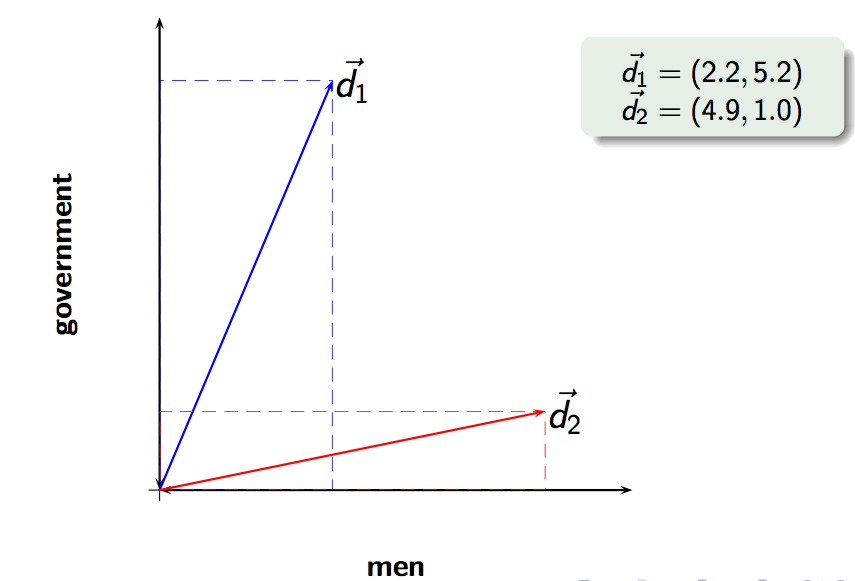
\includegraphics[width=.8\linewidth]{VSM-vectores.png}\\
  \end{center}

\end{frame}



%% \begin{frame}
%%  \frametitle{An example}
%% 
%%  \only<1>{
%%    \begin{example}
%%      \begin{itemize}
%%      \item Suppose the vocabulary has two terms $k_1 = \text{`men'}$, $k_2 =
%%        \text{`government'}$
%%      \item Two documents, $d_1$ and $d_2$ can be defined as, for instance
%%        \begin{itemize}
%%        \item $\vec{d_1} = (2.2,5.2)$
%%        \item $\vec{d_2} = (4.9,1.0)$
%%        \end{itemize}
%%      \end{itemize}
%%    \end{example}
%%  }
%% 
%%  \only<2>{
%%    \begin{columns}[t]
%% 
%%      \column{0.7\textwidth}
%% 
%%      \begin{pspicture}(-2,-2)(6,6) \psaxes[unit=6]{<->}(1,1)
%%        \rput{90}(-1.2,3){\textbf{government}} \rput(3,-1){\textbf{men}}
%% 
%%        \rput(2.2,5.2){\rnode{D1}{\Large ~~~$\vec{d_1}$}}
%%        \psframe[linestyle=dashed,linecolor=Blue,linewidth=0.1mm](D1)
%%       \psline[linecolor=Blue]{->}(D1)
%%        \rput(4.9,1.0){\rnode{D2}{\Large ~~~$\vec{d_2}$}}
%%       \psframe[linestyle=dashed,linecolor=Red,linewidth=0.1mm](D2)
%%       \psline[linecolor=Red]{->}(D2)
%%     \end{pspicture}
%%      \column{0.3\textwidth}
%% 
%%       \begin{exampleblock}{}
%%         \centering
%%         $\vec{d_1} = (2.2,5.2)$\\
%%         $\vec{d_2} = (4.9,1.0)$
%%       \end{exampleblock}
%% 
%%    \end{columns}
%%  }
%% 
%% \end{frame}

% ------------------------------------------------------------

\begin{frame} \frametitle{Defining Document Vectors}
  
  \begin{block}{Two questions are still unanswered:}
    \begin{enumerate}
    \item How do we define term weights?
    \item How do we compare documents to queries?
    \end{enumerate}
  \end{block}

\end{frame}

% ------------------------------------------------------------

\begin{frame} \frametitle{Defining Term Weights --- TF}

  \begin{block}{Term frequency}
    Term frequency is a measure of term importance \emph{within a document}
  \end{block}

  \begin{definition}
    Let $N$ be the total number of documents in the system and $n_i$ be the
    number of documents in which term $k_i$ appears. The \alert{normalized
      frequency} of a term $k_i$ in document $d_j$ is given by:
    \begin{displaymath}
      f_{i,j} = \frac{freq_{i,j}}{\max_l freq_{l,j}}
    \end{displaymath}
    where $freq_{i,j}$ is the number of occurrences of term $k_i$ in document
    $d_j$.
  \end{definition}

\end{frame}

% ------------------------------------------------------------

\begin{frame} \frametitle{Defining Term Weights --- IDF}

  \begin{block}{(Inverse) Document frequency}
    Document frequency is a measure of term importance \emph{within a
      collection}
  \end{block}

  \begin{definition}
    The \alert{inverse document frequency} of a term $k_i$ is given by:
    \begin{displaymath}
      idf_i = \log \left( \frac{N}{n_i} \right)
    \end{displaymath}
  \end{definition}

\end{frame}

% ------------------------------------------------------------

\begin{frame}
  \frametitle{Defining Term Weights --- TF-IDF}

  \begin{definition}
    The weight of a term $k_i$ in document $d_j$ for the vector space model is
    given by the \alert{tf-idf} formula:
    \begin{displaymath}
      w_{i,j} = f_{i,j} \times \log \left( \frac{N}{n_i} \right)
    \end{displaymath}
  \end{definition}

\end{frame}

\begin{frame}
  \frametitle{Components of TF-IDF}

  Different TF-IDF formulations consider alternative approaches for the TF and IDF components, and also for normalizing the resulting vectors.
  \begin{center}
    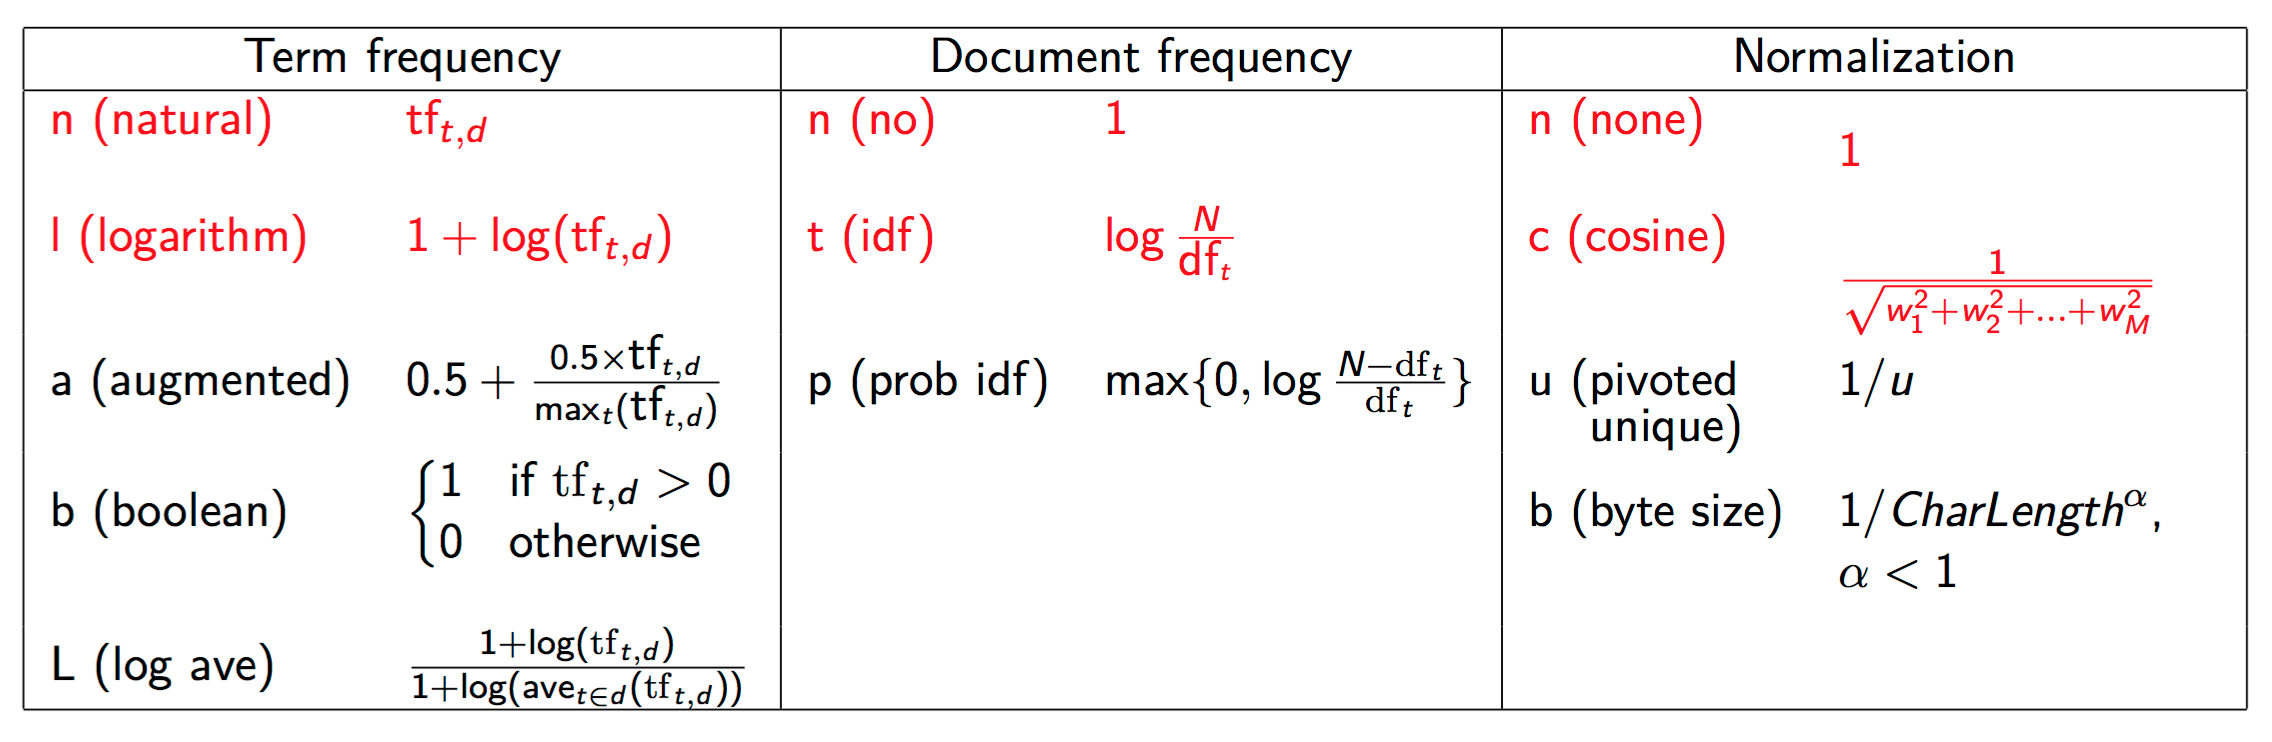
\includegraphics[width=.9\linewidth]{tfidf-variants.png}\\
  \end{center}

\end{frame}

% ------------------------------------------------------------

\begin{frame} \frametitle{Document Similarity}

  \begin{block}{}
    \begin{itemize}
    \item Similarity between documents and queries is a measure of the
      correlation between their vectors
    \item Documents/queries that share the same terms, with similar weights,
      should be more similar
    \item Thus, as similarity measure, we use the \alert{cosine of the angle
        between the vectors}
      \begin{displaymath}
        %psframebox not supported in pdflatex
        %\psframebox[linestyle=dashed,linecolor=Blue]{
          sim(d_j,q) =
          \frac{\vec{d_j}\cdot\vec{q}}{|\vec{d_j}|\times|\vec{q}|} =
          \frac{\sum_{i=1}^{t}w_{i,j} \times w_{i,q}}
               {\sqrt{\sum_{i=1}^{t}w_{i,j}^2} \times \sqrt{\sum_{i=1}^{t}w_{i,q}^2}}
        %}
      \end{displaymath}
    \end{itemize}
  \end{block}
\end{frame}

% ------------------------------------------------------------

%% esta frame n�o funciona com pslatex; substitui a seguinte 
%% formata com pdflatex

\begin{frame}
  \frametitle{An Example}

  \begin{center}
    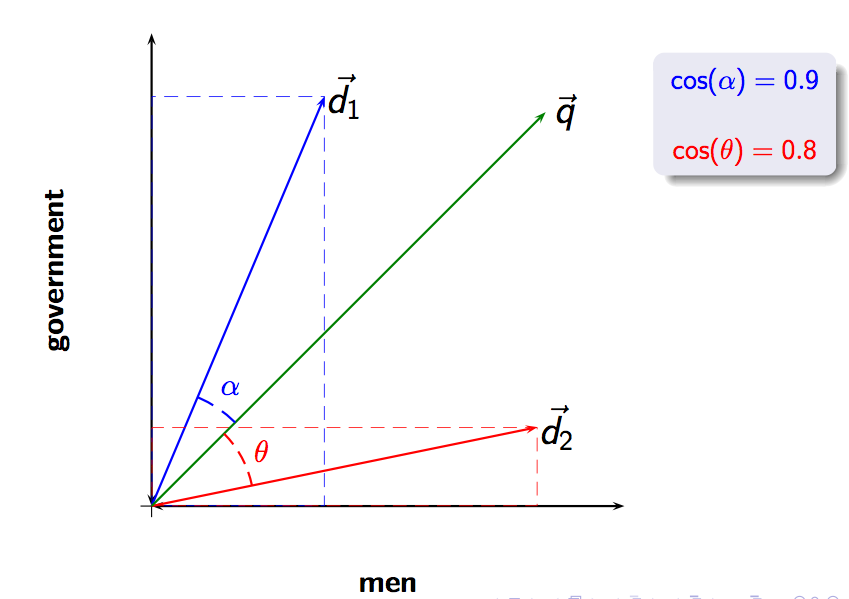
\includegraphics[width=.8\linewidth]{VSM-cosenos.png}\\
  \end{center}

\end{frame}



%% esta frame n�o funciona com pdflatex; substitu�da pela anterior

%% \begin{frame}
%%  \frametitle{An Example}
%% 
%%  \begin{columns}[t]
%% 
%%    \column{0.8\textwidth}
%% 
%%    \begin{pspicture}(-2,-2)(6,6) \psaxes[unit=6]{<->}(1,1)
%%      \rput{90}(-1.2,3){\textbf{government}} \rput(3,-1){\textbf{men}}
%% 
%%      \rput(2.2,5.2){\rnode{D1}{\Large ~~~$\vec{d_1}$}}
%%      \psframe[linestyle=dashed,linecolor=Blue,linewidth=0.1mm](D1)
%%      \psline[linecolor=Blue]{->}(D1)
%% 
%%      \rput(4.9,1.0){\rnode{D2}{\Large ~~~$\vec{d_2}$}}
%%      \psframe[linestyle=dashed,linecolor=Red,linewidth=0.1mm](D2)
%%      \psline[linecolor=Red]{->}(D2)
%% 
%%      \rput(5,5){\rnode{Q}{\Large ~~~$\vec{q}$}}
%%      \psline[linecolor=Green]{->}(Q)
%% 
%%      \psarc[linestyle=dashed,linecolor=Blue](0,0){1.5}{45}{67}
%%      \psarc[linestyle=dashed,linecolor=Red](0,0){1.3}{11.5}{45}
%% 
%%      \rput(1,1.5){\textcolor{Blue}{$\alpha$}}
%%      \rput(1.4,0.7){\textcolor{Red}{$\theta$}}
%%    \end{pspicture}
%% 
%%    \column{0.2\textwidth}
%% 
%%    \begin{block}{}
%%     \centering
%%     \small
%%     \textcolor{Blue}{$\cos(\alpha) = 0.9$}\\[3ex]
%%     \textcolor{Red}{$\cos(\theta) = 0.8$}\\
%%   \end{block}
%%  \end{columns}
%% \end{frame}

% ------------------------------------------------------------

\begin{frame}  \frametitle{The Vector Space Model}

  \begin{block}{Why is it so good?}
    \begin{itemize}
    \item Simple model, based on linear algebra
    \item Term weights are not binary
    \item Allows computing a continuous \emph{degree of similarity} between
      queries and documents
    \item Thus, allows \emph{ranking} documents according to their possible
      relevance
    \end{itemize}
  \end{block}
\end{frame}

\begin{frame}{Improving the VSM (1)}

\begin{block}{The BM25 Model}

    Consider not only the term frequency and inverse document frequency heuristics, but also the \emph{document length as a normalization factor} for the term frequency

    \begin{displaymath}
          TF_{i,j} = \frac{f_{i,j} \times (k_1 + 1)}
                                  {f_{i,j} + k_1 \times \left( 1-b+b\frac{|d_j|}{avgdl} \right)}
    \end{displaymath}
    \begin{displaymath}
        IDF_i = \log\frac{N - n_i + 0.5}{n_i + 0.5}
    \end{displaymath}
    \begin{displaymath}
          sim(d_j,q) =
          \sum_{i \in q} IDF_i \times TF_{i,j} 
    \end{displaymath}

    ~\\
    To be detailed in the next lecture
\end{block}
    
\end{frame}

\begin{frame}{Improving the VSM (2)}
\begin{block}{Latent Semantic Indexing}
\begin{itemize}
\item Find a low-rank approximation of the matrix which describes the occurrences of terms in documents

\begin{itemize}
\item Singular Value Decomposition
\item Compare the documents in the low-dimensional space
\end{itemize}
\item The consequence of the rank lowering is that some dimensions are combined (e.g., \emph{mitigates the problem of identifying synonymy})
\end{itemize}
\begin{itemize}
\item To be detailed latter in the course
\end{itemize}
\end{block}
\end{frame}


% ------------------------------------------------------------

\section{Probabilistic Models}
\label{sec:probabilistic}

\begin{frame}  \frametitle{Probabilistic Models for IR}
\begin{block}{}
TF-IDF and VSM produces sufficiently good results in practice, but often criticized for being \emph{too ad-hoc} or \emph{not principled}
\end{block}
\begin{itemize}
\item Typically outperformed by probabilistic retrieval models and statistical language models in IR benchmarks
\item Probabilistic retrieval models
   \begin{itemize}
   \item use generative models of documents as bags-of-words 
   \item explicitly model probability of relevance $P(R|d_j,q)$
   \item probabilistic justification for TF-IDF-like approaches
   \end{itemize}
\item Statistical language models
   \begin{itemize}
   \item use generative models of documents and queries as sequences-of-words
   \item consider likelihood of generating query from document model or divergence of document model and query model
   \end{itemize}
\end{itemize}
\end{frame}

\begin{frame}  \frametitle{Probabilistic Retrieval Models}
    \begin{block}{Bayes optimal decision rule for set retrieval}
      \begin{displaymath}
        %psframebox not supported in pdflatex
        %\psframebox[linestyle=dashed,linecolor=Blue]{
          d_j \text{~~is relevant iff~~} P(R|d_j,q) > P(\overline{R}|d_j,q)
        %}        
      \end{displaymath}
    \end{block}
    \begin{itemize}
    \item Model the IR problem in a probabilistic framework
    \item Estimate the probability of document $d_j$ being relevant to the user that that submited the query $q$
    \item When considering ranked retrieval, present documents in decreasing order of their estimated probability of relevance
    \end{itemize}
\end{frame}

\begin{frame}  \frametitle{Binary Independence Model (BIM)}
  \begin{block}{Simplifying assumptions for $P(R|d_j,q)$}
    \begin{itemize}
    \item A simple probabilistic model can assume that:
      \begin{enumerate}
      \item probability depends only on query and document
      \item there is a subset $R$ of relevant documents
      \item index terms are independent
      \item non-query terms are equally likely to appear in relevant and non-relevant documents
      \end{enumerate}
    \item Use \emph{binary term weights}
      \begin{itemize}
      \item documents and queries as binary term incidence vectors
      \item terms not appearing in the query do not affect the ranking
      \end{itemize}
    \end{itemize}
  \end{block}

\end{frame}

% ------------------------------------------------------------

\begin{frame} \frametitle{Document Query Similarity}

  \begin{block}{}
    \begin{itemize}
    \item As a similarity measure, we can use the ratio between the probability of
      finding the relevant documents and the probability of finding the
      non-relevant documents
      \begin{displaymath}
        %psframebox not supported in pdflatex
        %\psframebox[linestyle=dashed,linecolor=Blue]{
          sim(d_j,q) = \frac{P(R|\vec{d_j},\vec{q})}{P(\overline{R}|\vec{d_j},\vec{q})}
        %}        
      \end{displaymath}
     \item Often refered to as the \emph{Retrieval Status Value (RSV)}
    \end{itemize}
  \end{block}
\end{frame}

% ------------------------------------------------------------

\begin{frame}[allowframebreaks]
  \frametitle{Similarity Probabilities}

  \begin{block}{Initial Equation}
    We can simplify the expression leveraging Bayes’ theorem and rank equivalence
    \small
    \begin{displaymath}
        sim(d_j,q) = \frac{P(R|\vec{d_j},\vec{q})}{P(\overline{R}|\vec{d_j},\vec{q})}
        = \frac{P(\vec{d_j},\vec{q}|R) \times P(R)}{P(\vec{d_j},\vec{q}|\overline{R}) \times
          P(\overline{R})}
        \sim \frac{P(\vec{d_j},\vec{q}|R)}{P(\vec{d_j},\vec{q}|\overline{R})}
     \end{displaymath}
  \end{block}

  \begin{block}{Assuming term independence...}
    \footnotesize
    \begin{displaymath}
      sim(d_j,q) \sim \frac{
        (\Pi_{g_i(\vec{d_j})=g_i(\vec{q})=1}P(k_i|R))\times(\Pi_{g_i(\vec{d_j})=0 \wedge g_i(\vec{q})=1}P(\overline{k_i}|R))
      }{
        (\Pi_{g_i(\vec{d_j})=g_i(\vec{q})=1}P(k_i|\overline{R}))\times(\Pi_{g_i(\vec{d_j})=0 \wedge g_i(\vec{q})=1}P(\overline{k_i}|\overline{R}))}
    \end{displaymath}
  \end{block}

  \begin{block}{Taking $\log$s and removing constant factors...}
    \small
    \begin{displaymath}      
      sim(d_j,q) = \sum_{i=1}^t w_{i,q} \times w_{i,j} \times
      \left(
        \log\frac{P(k_i|R)}{1-P(k_i|R)} + \log\frac{1-P(k_i|\overline{R})}{P(k_i|\overline{R})}
      \right)
    \end{displaymath}
  \end{block}

  \begin{block}{Blind assumptions}
    \begin{displaymath}
      \begin{array}{rcl}
        P(k_i|R) &=& 0.5\\
        P(k_i|\overline{R}) &=& \frac{n_i}{N}\\
      \end{array}
    \end{displaymath}
    \begin{itemize}
    \item $P(k_i|R)$ reflects that we have no information about relevant documents (i.e., each query term is equally likely to occur in a relevant document)
    \item $P(k_i|\overline{R})$ under the assumption that \# relevant documents $<$ \# documents
    \end{itemize}
  \end{block}

  \begin{block}{After document retrieval or leveraging training data...}
    \begin{itemize}
    \item Let $V$ be the number of returned documents (i.e., number of documents estimated to be relevant)
    \item Let $V_i$ be the number of returned docs with term $k_i$
    \end{itemize}
    \begin{displaymath}
      \begin{array}{rcl}
        P(k_i|R) &=& \frac{V_i}{V}\\
        P(k_i|\overline{R}) &=& \frac{n_i - V_i}{N - V}\\
      \end{array}
    \end{displaymath}    
  \end{block}
  
  \begin{block}{Avoiding small values when using blind assumptions...}
    \begin{itemize}
    \item With \emph{zero counts} probability is not well-defined
    \item Maximum likelihood estimates do not work for rare events
    \item To avoid zeros add 0.5 to each count (expected likelihood estimation) or use a different type of smoothing
    \end{itemize}
    \begin{displaymath}
      \begin{array}{rcl}
        P(k_i|R) &=& 0.5\\
        P(k_i|\overline{R}) &=& \frac{n_i + 0.5}{N + 0.5}\\
      \end{array}
    \end{displaymath}   
  \end{block}
  
  \begin{block}{Avoiding small values with estimates after retrieval...}
    \begin{displaymath}
      \begin{array}{rcl}
        P(k_i|R) &=& \frac{V_i + \frac{n_i}{N}}{V + 1}\\
        P(k_i|\overline{R}) &=& \frac{n_i - V_i + \frac{n_i}{N}}{N - V + 1}\\
      \end{array}
    \end{displaymath}    
  \end{block}
\end{frame}

% ------------------------------------------------------------

\begin{frame} \frametitle{Problems of this Simple Probabilistic Model}
  \begin{block}{}
    \begin{itemize}
    \item There is no accurate estimate for the first run probabilities
    \item Index terms are not weighted
    \item Terms are assumed mutually independent
    \end{itemize}
  \end{block}
  \begin{block}{}
    In fact, \emph{many different probabilistic retrieval models} have been proposed, some addressing the aforementioned limitations!
  \end{block}
\end{frame}

% ------------------------------------------------------------

\begin{frame}[allowframebreaks]
\frametitle{Another Look at the BIM}

  \begin{block}{Recall the log odds ratio for computing RSV}
    \small
    \begin{displaymath}      
      sim(d_j,q) = \sum_{i=1}^t w_{i,q} \times w_{i,j} \times
      \left(
        \log\frac{P(k_i|R)}{1-P(k_i|R)} + \log\frac{1-P(k_i|\overline{R})}{P(k_i|\overline{R})}
      \right)
    \end{displaymath}
  \end{block}
  
  \begin{block}{Denoting $p_i = P(k_i|R)$ and $u_i = P(k_i|\overline{R})$}
    \small
    \begin{displaymath}      
      sim(d_j,q) = \sum_{i=1}^t w_{i,q} \times w_{i,j} \times
      \left(
        \log\frac{p_i}{1 - p_i} + \log\frac{1 - u_i}{u_i}
      \right)
    \end{displaymath}
  \end{block}
		
  \begin{block}{With the blind estimates, does the equation look familiar?}
    \begin{displaymath}  
    P(k_i|R) = p_i = 0.5
    \end{displaymath}
    
    \begin{displaymath}  
    P(k_i|\overline{R}) = u_i = \frac{n_i}{N}
    \end{displaymath}
    
    \begin{center}
    Replacing $p_i$ and $u_i$ in the previous equation...
    \end{center}
    
     \begin{displaymath}      
       \log\frac{p_i}{1 - p_i} = 0
    \end{displaymath}
    
    \begin{displaymath}      
       \log\frac{1 - u_i}{u_i} = \log\frac{N - n_i}{n_i} \approx \mathbf{\log \left( \frac{N}{n_i} \right)}
    \end{displaymath}
  \end{block}
  
  \begin{block}{}
    \begin{itemize}
    \item The BIM can be seen as TF-IDF with binary term frequencies and logarithmically dampened inverse document frequencies
    \item The score for document $d$ is just \emph{IDF weighting of the query terms present in the document}
    \end{itemize}
	\begin{displaymath}  
	sim(d_j,q) = \sum_{i=1}^t w_{i,q} \times w_{i,j} \times \log \left( \frac{N}{n_i} \right)
	\end{displaymath}
    \begin{itemize}
    \item Alternative formulation using smoothing
    \end{itemize}
	\begin{displaymath}  
	sim(d_j,q) = \sum_{i=1}^t w_{i,q} \times w_{i,j} \times \log \left( \frac{N - n_i + 0.5}{n_i + 0.5} \right)
	\end{displaymath}
   \end{block}
\end{frame}

\begin{frame} \frametitle{The Okapi BM25 Model (1)}
\begin{itemize}
\item Inspired by the BIM probabilistic formulation
\item Considering an alternative for term weighting
\item Captures various aspects in a simple formula, tuning each component
    \begin{itemize}
    \item Inverse Document Frequency (IDF)
    \item Term Frequncy (TF)
    \item Document length 
    \item Query term fequency {\it (in some formulations)}
    \end{itemize}
\item BM25 (BestMatch25) is an effective and widely used model
\end{itemize}
\end{frame}

\begin{frame} \frametitle{The Okapi BM25 Model (2)}
\begin{block}{The BM25 Model}
    \begin{displaymath}
          TF_{i,j} = \frac{f_{i,j} \times (k_1 + 1)}
                                  {f_{i,j} + k_1 \times \left( 1-b+b\frac{|d_j|}{avgdl} \right)}
    \end{displaymath}
    \begin{displaymath}
        IDF_i = \log\frac{N - n_i + 0.5}{n_i + 0.5}
    \end{displaymath}
    \begin{displaymath}
          sim(d_j,q) =
          \sum_{i \in q} IDF_i \times TF_{i,j} 
    \end{displaymath}
\end{block}
\begin{itemize}
\item Postulates Poisson (or 2-Poisson-mixture) distributions for terms, instead of Binomial distributions as in BIM
\item Parameters $k_1$ and $b$ need to be tuned
\begin{itemize}
\item $k_1$ controls impact of term frequency
\item $b$ controls impact of document length
\item Setting $k_1 = 1.5$ and $b = 0.75$ are common defaults
\end{itemize}
\end{itemize}
\end{frame}

% ------------------------------------------------------------

\begin{frame} \frametitle{Probabilistic Language Models}
  \begin{block}{}
    \begin{itemize}
\item Another simple probabilistic retrieval model
\item Each document $d$ is treated as (the basis for) a \emph{probabilistic language model}
\item Given a query $q$ rank documents based on $P(d|q)$
\begin{equation*}
P(d|q) = \frac{P(d) \times P(q|d)}{P(q)}
\end{equation*}
\item The evidence $P(q)$ is the same for all documents, so ignore
\item $P(d)$ is the prior
\begin{itemize}
\item often treated as the same for all $d$
\item  we can give a higher prior to ``high-quality'' documents (e.g., those with high PageRank -- to be seen latter)
\end{itemize}
\item $P(q|d)$ is likelihood, i.e. the probability of $q$ given $d$
    \end{itemize}
  \end{block}

\end{frame}
\begin{frame} \frametitle{How to compute $P(q|d)$}
  
  \begin{block}{}
  \scriptsize
    \begin{itemize}
    \item Conditional independence assumption
	\begin{equation*}
	P(q|d) = P(\{t_1,\ldots,t_{|q|}\}|d) = \prod_{1<=k<=|q|} P(t_k|d)
	\end{equation*}
    \item $|q|$ is length of $q$
    \item $t_k$ is the token occurring at position $k$ in $q$
    \end{itemize}
  \end{block}

  \begin{block}{}
    \scriptsize
    \begin{itemize}
    \item The above multinomial model is equivalent to:
	\begin{equation*}
	P(q|d) = \prod_{\text{distinct term~} t \in q} P(t_k|d)^{TF_{t,q}}
	\end{equation*}
	\item Component $TF_{t,q}$ is the term frequency of $t$ in $q$
    \item Parameters $P(t_k|d)$ computed through maximum likelihood estimates
	\end{itemize}
		\begin{equation*}
		P(t_k|d) = \frac{TF_{t_k,d}}{|d|}
		\end{equation*}
  \end{block}

\end{frame}

% MLE of multinomial: https://math.stackexchange.com/questions/421105/maximum-likelihood-estimator-of-parameters-of-multinomial-distribution

\begin{frame}
    \frametitle{Types of Language Models}

    \begin{itemize}
    \item The unigram language model (show before)
        \begin{displaymath}
            P(d) = P(t_1t_2t_3\ldots) = P(t_1)P(t_2)P(t_3)\cdots
        \end{displaymath}
    \item $n$-gram language models (e.g. \textit{bigram} language models)
        \begin{displaymath}
            P(d) = P(t_1t_2t_3\ldots) = P(t_1)P(t_2|t_1)P(t_3|t_2)\cdots
        \end{displaymath}
    \item More complex langue models, e.g. using \textit{probabilistic context-free grammars}
        \begin{itemize}
        \item Used for tasks like speech recognition , spelling correction , and machine translation
        \end{itemize}
    \end{itemize}
\end{frame}

\begin{frame} \frametitle{LM Retrieval and Na{\"i}ve Bayes}
    
    \begin{block}{}
    The next class will introduce a simple probabilistic document classifyer, known as the \emph{Na{\"i}ve Bayes} approach
    \end{block}
  
    \scriptsize
    \begin{itemize}
    \item We want to classify document $d$. \\ \emph{We want to classify a query $q$}
	\item Human-defined classes: e.g., politics, economics, sports. \\ \emph{Each document in the collection is a different class}
	\item Assume that $d$ was produced by the generative model. \\ \emph{Assume that $q$ was generated by a generative model}
    \item Which of the classes (= class models) is most likely to have generated the document $d$? \\ \emph{Which document (=class) is most likely to have generated the query $q$?}
    \item For which class do we have the most evidence? \\ \emph{For which document (as source for query) do we have the most evidence?}
	\end{itemize}

\end{frame}


% ------------------------------------------------------------

\section{Comparison of the Different Models}
\label{sec:comparison}

\begin{frame}  \frametitle{What makes these Models Work?}

\begin{block}{Three main term weighting normalization driving features:}
\begin{itemize}
\item TF - Term Frequency
\item IDF - Inverse Document Frequency
\item DL - Document Length
\end{itemize}
\end{block}
\end{frame}

\begin{frame}   \frametitle{Comparison of the Different Models}

  \begin{block}{}
    \begin{itemize}
    \item Boolean model is considered the weakest
    \item There is some controversy over which shows better performance: vector space or probabilistic
     \begin{itemize}
     \item Simple BIM is just IDF weighting of the terms
     \item BIM was originally designed for short catalog records of fairly consistent length, and it works reasonably in these contexts
     \item BM25 or language models offer a better performance (e.g., paying attention to term frequency and document length)
     \end{itemize}
    \item Nowadays, BM25 is perhaps the most widely used
    \end{itemize}
  \end{block}
\end{frame}

% ------------------------------------------------------------

\finalframe{Questions?}

\end{document}

%%% Local Variables: 
%%% mode: latex
%%% TeX-master: t
%%% End: 
